\chapter{SV Detection in Single Cells}
\label{sec:mosaicatcher}

Here, I present the current state of a project with the objective to develop a
computational method for \sv detection in Strand-seq data. This method is being
developed together with \jan and \ashley as well as with our collaborators
\david, \maryam, and \marschall from the Max-Planck Institute for Informatics,
Saarbrücken. \ashley and \jan conceived the general concept of \sv discovery
based on the signals provided by Strand-seq data. \marschall and \david
contributed analyses related to phasing and and improvements to the overall work
flow. \maryam developed the Bayesian classification approach described below.
Also work from \venla on \acl{sce} events was included into this method.
The main implementation and all other analyses, including figures, are my own.
At last, I would like to thank \balca, who provided the cell lines utilized for
demonstration purposes, and \landsdorp's lab, who carried out the Strand-seq
experiments on this cell line.





\section{Structural variants in the context of somatic mosaicism}
\label{sec:mosaic_mosaicism}

\todo{Write this section}
text text text text text text text text text text text text text text text
text text text text text text text text text text text text text text text
text text text text text text text text text text text text text text text





\section{\textsc{Mosaicatcher}: A novel approach for comprehensive SV detection in single-cell Strand-seq data}
\label{sec:mosaic_mc}

Strand-seq generates sequencing reads that are all of the same directionality
when they stem from the same homologue. As explained in \cref{sec:strandseq},
this is achieved by labeling and degrading the non-template strand of
actively replicating cells. When the resulting sequencing reads are mapped to a
reference assembly, they map either to the Watson (W) or Crick (C) strand. The
presence of two homologous chromosomes then leads to the presence WW, CC, or WC
chromosomes, which we call their \emph{inherited strand states}.
Here, I show how these unique characteristics of Strand-seq reveal the presence
of seven different \sv classes and demonstrate our computational method called
\mc that implements this idea.

%\afterpage{%
%    \clearpage%
%    \ifodd\value{page} \expandafter\afterpage \fi {%
    \begin{figure}[t!]                                             % cell BM160815_WT_007p1 from BM160815_WT.200000.pdf
        \captionsetup{type=figure}
        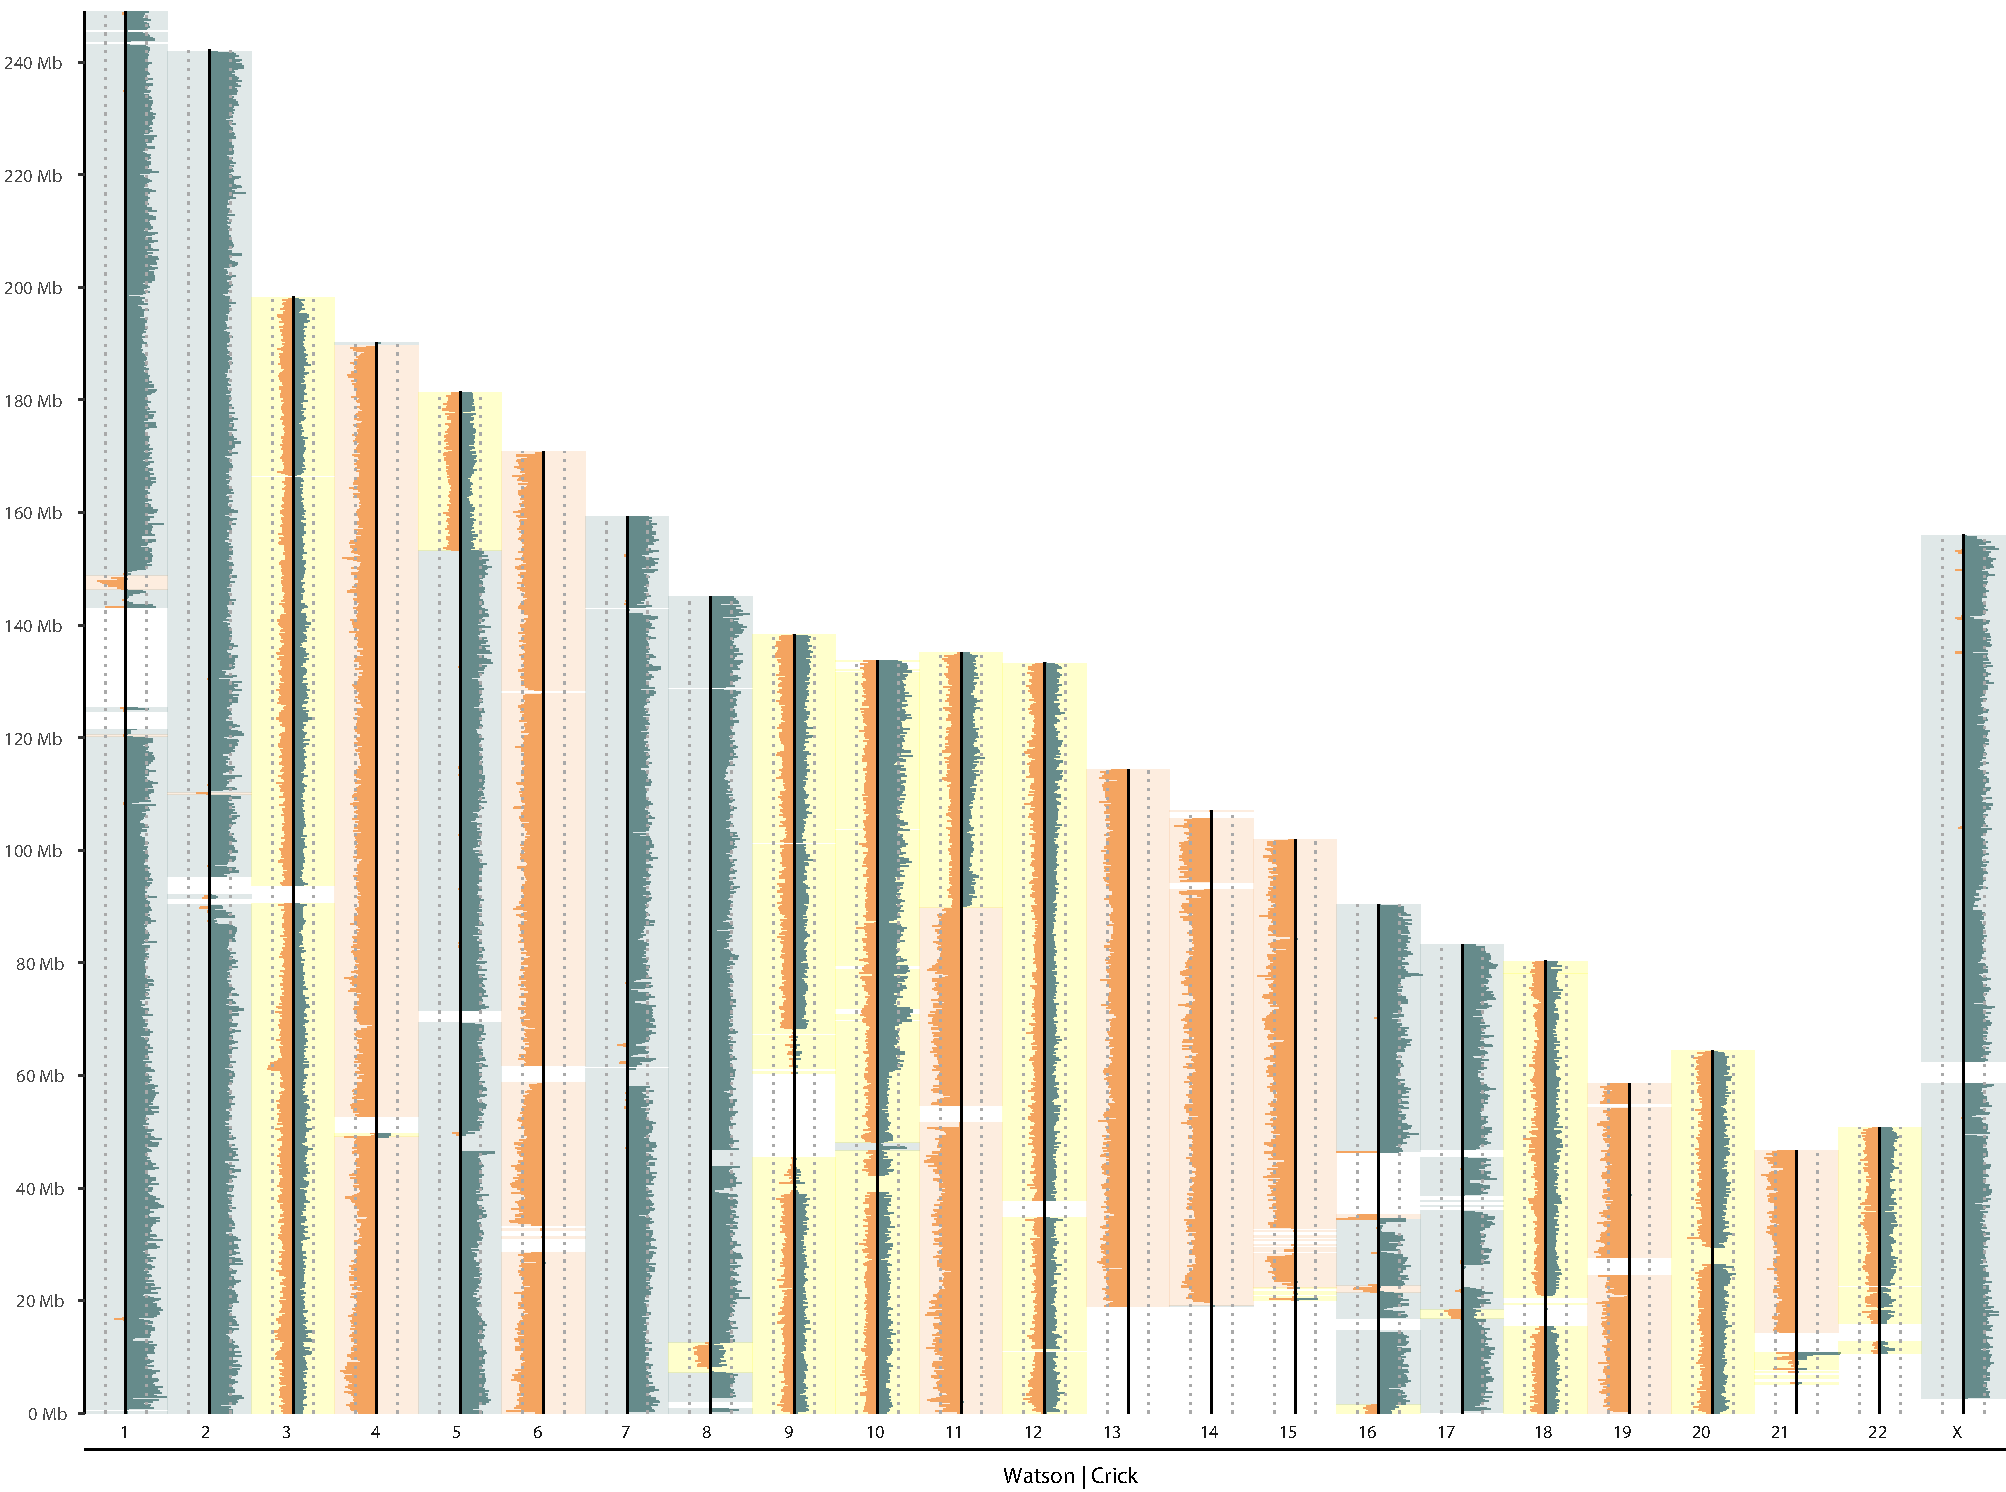
\includegraphics[width=\textplusmargin,inner]{ss_lib_rpewt.pdf}
        \figcap{ss_library}{Example of a single cell Strand-seq library}{
            Here, a single cell Strand-seq library of an \rpe-I wild type cell
            line is displayed using the plot function of \mc.
            Each vertical panel shows binned read counts of one chromosome, with
            the Watson strand on the left, in orange, and the Crick strand on
            the right in blue. In the cell shown here, each 200~kb-bin contains
            a median of 76 total reads, which is depicted by the
            dotted lines. Some regions, e.g. the centromere of chromosome 1 or
            the sub-telomeric regions of chromosomes 13--15 are not coverded by
            reads because of mappability issues; these bins are excluded from
            further analyses. The estimated strand inheritance state of each bin
            is color-coded in the background: blue for CC, orange for WW and yellow
            for WC. Chromosomes 5 and 11 carry \acp{sce}, which are visible by a
            change in the strand inheritance state that continues to the end of
            the chromosomes.}%
    \end{figure}
%    }}

\Cref{fig:ss_library} depicts Strand-seq data from a single cell of an \acf{rpe}
wild type cell line (courtesy by \balca and \landsdorp). This cell-wide overview
plot was generated using \mc and is typically the starting point for
an analysis of Strand-seq data. The procedure leading to this plot is outlined
briefly in \cref{sec:mosaic_method}.

An overview plot allows an initial judgment on the success, quality, and depth
of a Strand-seq library. In the cell shown here, reads aligning to either W or C
strand were binned at 200~kb resolution. The cell was sequenced at ample depth
(median 76 reads per bin), shows the Strand-seq characteristic strand
inheritance patterns (WW, CC, and WC chromosomes) and is of high quality, which
can be judged from the low number of reads on the opposite strand in WW or CC
cells and a fairly even coverage distribution. Experimental parameters
influencing the quality of Strand-seq libraries are discussed in detail by
\cite{Sanders2017}.

\Cref{fig:ss_library} further gives a first impression of genomic rearrangements
in this cell. For example, the region of WW reads at around 120~Mb on chromosome
1 reveals an inversion of that locus in respect to the reference assembly. The
most prominent alterations are visible on chromosomes 5 and 11, though. Here,
the strand inheritance states change at one position and remain consistent to
the end of the chromosome from there. These positions mark \acf{sce} events,
which are reciprocal exchanges between two identical sister chromatids and
which can be specifically measured using Strand-seq \citep{Falconer2012}.
\Acp{sce} occur randomly across the genome and must not be mistaken with other
classes of \acp{sv} for our purpose.





\subsection{Three signals within Strand-seq data are distinctive of SVs}
\label{sec:mosaic_concept}

Strand-seq libraries reveal the presence of large \Acl{sv}. This had been shown
for inversions in the past by \cite{Sanders2016}. Here, we determined seven
different \sv classes that can be revealed in Strand-seq data, five of which are
principally discernible within a single cell (deletion, duplication, inversion,
inverted duplication, \loh), and two that become apparent across a population of
cells (aneuploidy and translocation). These \sv classes can be distinguished
using three independent signals: (1) the normalized read coverage of a locus,
which corresponds to a diploid state (2N) in a non-affected locus.
(2) The strand ratio, i.e. the number of W reads over the number of C reads.
Alternatively, a fraction can be used here, for example the Watson fraction
W/(W+C). (3) Haplotype information. When whole-chromosome haplotypes are known
at sites of \acp{snv}, these alleles can be used to reason about potential
rearrangements. Sequencing reads overlapping such variants can be queried for
both their original homologue \emph{and} their strand direction.
Below I explain how we can utilize the combination of these signals to detect,
genotype and phase \acp{sv}. \Cref{fig:mosaic_examples} contains examples of
several \sv classes that we identified in \rpe cell lines.

\FloatBarrier
\begin{table}[t]%
\newcommand\ccb{\cellcolor{blue!10}}
\newcommand\cco{\cellcolor{orange!10}}
    \begin{adjustbox}{width=\textplusmargin,inner}%
    \begin{tabu} to \textplusmargin {X[l] c c c c l c c c c}
        \toprule
          & \multicolumn4{c}{WC chromosome} & & \multicolumn4{c}{WW chromosome} \\
         \cmidrule{2-5} \cmidrule{7-10}
          & & & \multicolumn2{c}{Haplotype} & & & & \multicolumn2{c}{Haplotype} \\
        \cmidrule(lr){4-5} \cmidrule(lr){9-10}
         & Cov. & W.f. & \emph{W} & \emph{C} & & Cov. & W.f. & \emph W & \emph{C} \\
        \midrule
        Reference allele             &      2N &      50\% & $h_1$   & $h_2$     & &      2N &      100\% & $h_1 + h_2$     & - \\
        Deletion of $h_1$            &      1N &       0\% & -       & $h_2$     & & \ccb 1N & \ccb 100\% & $h_2$           & - \\
        Deletion (homozygous)        &      0N &         - & -       & -         & &      0N &          - & -               & - \\
        Duplication of $h_1$         &      3N &      66\% & $2 h_1$ & $h_2$     & & \ccb 3N & \ccb 100\% & $2 h_1 + h_2$   & - \\
        Duplication (homozygous)     &      4N &      50\% & $2 h_1$ & $2 h_2$   & &      4N &      100\% & $2 h_1 + 2 h_2$ & - \\
        Inversion of $h_1$           &      2N &       0\% & -     & $h_1 + h_2$ & & \ccb 2N & \ccb  50\% & $h_2$ & $h_1$       \\
        Inversion (homozygous)       & \cco 2N & \cco 50\% & $h_2$   & $h_1$     & &      2N &        0\% & -     & $h_1 + h_2$ \\
        Inverted duplication ($h_1$) & \cco 3N & \cco 33\% & $h_1$ & $h_1 + h_2$ & & \ccb 3N & \ccb  66\% & $h_1 + h_2$ & $h_1$ \\
        \bottomrule
    \end{tabu}
    \end{adjustbox}
    \tabcap{mosaic_sv_signals}{Distinct signatures of focal SVs in Strand-seq
    data}{SVs can be identified based on three separate signatures of Strand-seq
    data: the total read coverage (\emph{Cov.}), the strand ratio---here shown
    as Watson fraction (\emph{W.f.}), and the presenece of haplotype-tagging
    \acp{snv} on each strand (\emph{Haplotpye}). In this table I show how the
    various focal \sv types can be inferred from these signals. This is different
    for WC chromosomes than for WW or CC chromosomes. For the sake of simpliciy,
    the table only shows the WW case and assumes heterozygous variants to affect
    haplotype $h_1$. Entries in orange are \sv classes that cannot be
    distinguished unambigously using only coverage and Watson fraction.
    Specifically, a homozygous inversions remain hidden in WC cells and an
    inverted duplication of $h_1$ cannot be distinguished from a duplication of
    $h_2$. Entries marked in blue cannot be phased based on coverage and Watson
    fraction alone. However, all these cases can be disentangled when
    haplotype-resolved \acp{snv} are available or by integrating information
    across several cells that share an \sv.}
\end{table}

\paragraph{Deletions and duplications}
\Acp{cnv} alter the total read coverage of an affected locus. A deletion
decreases the coverage from 2N to 1N, i.e. by a factor of two, and is hence
typically easier to detect---the same has been observed for other read
depth-based \sv callers. Duplications, which increase copy number to 3N, alter
the read depth only by a factor of 1.5 compared to the reference state.
Homozygous duplications increase the copy number even to 4N. Homozygous
deletions are marked by a complete absence of reads. They thus provide the
strongest change in read depth, with the only caveat that they resemble regions
of low mappability such as the centromere on chromosome 1. Homozygous deletions
are hence best studied in the presence of a control sample that does not carry
the deletion.

In contrast to classic read depth analysis, Strand-seq additionally provides
strand information. For example, a heterozygous deletion in a WC chromosome will
only lack reads on one of the strands. Similarly, a heterozygous duplication
will increase coverage only on one strand. In a WW or CC cell, strand
information does not add supportive evidence, but when phased \acp{snv} are
available, only one homologue will be deleted/duplicated.
\Cref{tab:mosaic_sv_signals} summarizes in detail how these signals
allow to differentiate the focal \sv classes that I cover here.

\paragraph{Copy-neutral variants}
Inversions do not change copy number, but become visible as a change in strand
ratio. A heterozygous inversion in a WW cell, for example, switches the strand
state to WC within the inverted locus. In a WC cell, it becomes WW or CC. Again,
in the WC cell the inversion can be phased trivially based on strand
directionality, whereas in the WW or CC case further \snv information has to be
consulted for phasing. A homozygous inversion is a special case: It changes a WW
chromosome into CC, making the locus clearly stand out, but it cannot be
observed within a WC cell. This is because both alleles change their strand
state, leading again to a WC region. This case can be disentangled with the help
of phased \acp{snv} or by observation of a population of cells
(\cref{tab:mosaic_sv_signals}).

Another copy-neutral \sv is \loh. In a \loh event, one homologue is
``overwritten'' by the other homologue, leading to extended regions of
homozygousity. To reveal \loh, alleles of\acp{snv} must be assessed. We recently
found independent regions of \loh within several cells of a lymphoblastoid cell
line (unbublished data)---all the work on haplotype information within this
project was spearheaded by \david and will hence not be covered in this
dissertation.

\paragraph{Complex variants}
Complex variants can partly be discovered in Strand-seq data, too. We chose
inverted duplications as a particular candidate, as this class has been found to
be abundant both on the small (\cref{sec:balancer}) as well as on the large
scale \citep{Chaisson2017}. As \cref{tab:mosaic_sv_signals} shows, inverted
duplications are marked by an increase in copy number as well as a flip in
strand orientation. In a WC cell, such an event cannot be distinguished from a
normal duplication unless \acp{snv} are available. \Cref{fig:mosaic_examples}
includes an example of an inverted duplication within an \rpe wild type cells.

\figuretextplusmargin[t!]{mosaic_sv_examples.pdf}{mosaic_examples}{Examples of SVs
    in RPE cells}{Strand-specific count data in 100~kb bins (Watson left, orange
    and Crick right, blue) are shown in several chromosomal regions of \rpe cells.
    \textbf{A:} Four loci of three cells each highlight four examples of focal
    \acp{sv} that could be identified in Strand-seq libraries. The affected
    loci (marked by dashed lines) show the characteristic changes in read
    coverage and strand state that were described in \cref{tab:mosaic_sv_signals}.
    \textbf{B:} A copy number gain of the q-arm of chromosome 10 is visible. The
    strand state of the extra copy correlates with the strand inheritance
    pattern of chromosome X (same cells for both chromosomes shown). This
    observation is best explained by an imbalanced translocation, as shown in
    the schematic.
    \textbf{C:} Five chromosomes of cells from the tetraploid RPE C29 cell line
    (courtesy by \balca and \landsdorp) were selected to represent the five
    possible strand inheritance patterns in a tetraploid cell: WWWW, WWWC, WWCC,
    WCCC, and CCCC.}


\paragraph{Aneuploidy}
In a Strand-seq experiment, each homologue of a chromosome is sequenced in
either W or C orientation. This fundamental property remains valid even in the
presence of more than two homologues. In a tetraploid cell, for example, a
chromosome is inherited in any one of five states: WWWW, WWWC, WWCC, WCCC, or
CCCC. By looking across a population of cells, Strand-seq can disclose the
ploidy of each chromosome, assuming it is not heterogeneous across cells
(\cref{fig:mosaic_examples}). A
usual way to estimate ploidy from \mps data is to assess the \baf of a bulk
sample---in a tetraploid chromosome, some \acp{snv} will be present at ratios of
25 or 75\%. Interestingly, Strand-seq detects ploidy even in the complete
absence of homologue-speicific variants, for example in cells with multiple
copies of the same homologue such as the CHM1 cell line \citep{Steinberg2014}.
To the best of our knowledge, this cannot be achieved by any other method.

\paragraph{Translocations}
At last, also translocations can be revealed using Strand-seq.  A reciprocal
translocation would alter the strand inheritance state of two chromosomes
simultaneously: An exchange between a WW and a CC chromosome would switch the
strand inheritance pattern into WC in both these chromosomes. However, such
changes in strand state can initially not be distinguished from randomly
occurring \sce events. This is why a correlated change between two chromosomes
must be observed across several cells to find translocations. In the \rpe wild
type cell line (\cref{fig:mosaic_examples}), we report an \emph{imbalanced}
translocation between chromosomes 10 and X, which had been noted
beforehand\footnote{In the description of the commercially available
    ``hTERT RPE-1'' cell line, a derivative of X is recognized, but chromosome
    10 is not mentioned. Source: \url{https://www.lgcstandards-atcc.org/Products/All/CRL-4000.aspx}}.
Here, chromosome 10 shows an increase in copy number on the q-arm that seems not
to be consistently on the same strand across cells. However, the strand
inheritance state of the extra copy perfectly matches the strand inheritance
state of chromosome X. This suggests that the extra copy of chromosome 10 is
linked physically to chromosome X. By correlating strand states across
chromosomes in this way, translocations can be discovered. The very same idea
has been used to assign unmapped contigs of the reference assembly to
chromosomes \citep{Hills2013}.







\FloatBarrier
\subsection{Automatd SV detecting}
\label{sec:mosaic_method}

In order to capture this spectrum of \sv classes, my collaborators and I
designed a computational approach for \sv calling from Strand-seq data.
This approach is implemented in a tool called \mc, which is currently being
developed. The core principle consists of the three steps (1) binning, (2)
segmentation, and (3) classification and is explained below. My code for the
first two steps is available online at
\url{https://github.com/friendsofstrandseq/mosaicatcher}.
The third part is being maintained by \maryam and can be found at
\url{https://github.com/friendsofstrandseq/MaRyam}. At last, the combined
workflow is available at \url{https://github.com/friendsofstrandseq/pipeline}.

\paragraph{Binning}
Strand-seq data is extremely sparse: the best libraries currently produced
contain around 300 reads per Megabases \citep{Chaisson2017,Sanders2017}. In
order to work with sparse data, I apply a binning scheme that summarizes
sequencing reads in windows of a given size, e.g. 50~kb. Alternatively, these
bins can have variable sizes (dynamic-width bins) to accommodate for regions of
low mappability. The transformation to binned counts allowed us to apply a
statistical model to estimate the expected number of reads per
bin---specifically, we utilized a \nb distribution, as I describe
later. Prior to binning, sequencing reads are filtered for low mapping quality
(a minimum score of 10 by default), supplementary alignments, and \pcr duplicates.
Also I only each read pair was counted only once to avoid double-counting of
sequenced fragments. I utilized the \htslib library within my implementation
to efficiently read and filter sequencing data.

Given the strand-specific binned counts, I implemented a plot function to
generate figures such as \cref{fig:ss_library}. At first, bins that are
consistently too low or high across all cells are masked: this is typically the
case in centromeric or telomeric regions. Further, I designed a classifier to
distinguish WW, WC, and CC states of each bin. This classifier is supposed to
tell the class of each bin based on its strand-specific read counts, but it
should further smoothen out fluctuations in single bins.
To achieve this, I implemented a \hmm with a multivariate \nb
emission distribution. The transition probability of the \hmm is chosen
according the expected number of \acp{sce} within a cell (e.g. 10 transitions
across all chromosomes). The output of this \hmm is used as background color in
aforementioned overview plots.

\paragraph{Segmentation}
The second step towards \sv calling is to detect the boundaries of potential
\acp{sv}. This had been done in the past by merging data of all cells in a
strand-aware fashion and detecting boundaries within the merged signal
\citep{Sanders2016}. However, this approach has the disadvantage that it can
mask subclonal variants, especially the ones at low allele frequency that we
are particularly interested in. Boundaries have also been determined within
single cells separately, e.g. based on an \hmm \citep{Bakker2016}. However, this
leads to the subsequent challenge of forming consensus boundaries across the
cells. Instead, I explored multivariate segmentation algorithms that consider
all cells simultaneously, yet still recognize them as individual cells. This is
further elaborated in \cref{sec:mosaic_segmentation}. Notably, the segmentation
algorithm is expected to provide potential \sv breakpoints, which are then
tested in the subsequent step. Thus, in order increase sensitivity, we allow the
segmentation to slightly overpredict boundaries.

\figurearbitrary[t!]{0.5}{mosaic_rpe_mean_var.pdf}{mean_var}{Mean variance
    relationship of binned read counts}{Each dot represents one cell of the
    \rpe-1 wild type cell line. Shown here are the mean number of reads per
    200~kb-bin vs. their variance. In a theoretical \nb distribution, mean and
    variance show a perfectly linear relationship with a slope $p$. In real data,
    we estimate $p$ by fitting a line without intercept.}

\paragraph{Classification} The third and final step is to test segments for the
presence of \acp{sv} (theory and implementation contributed by \maryam; figures
from me). In order to classify segments into either a \sv or non-\sv state, we
employ an elaborate Bayesian model based on \acl{nb} distributions.
Specifically, we model the read coverage in each strand by a \nb distribution,
which is adjusted to capture the expected number of reads within a given region.
Both strands combined yield a joint distribution for all possible strand
combinations, i.e. WW, WC, or CC, inclusing also abnormal states such as C, WWC,
and so on. Each of these joint strand states can then be interpreted in respect
to the expected state in the chromosome and cell. For example, a WC state would
signify a heterozygous inversion if it occurred on a WW chromosome, but no \sv
(or a homozygous inversion!) if it occurred on a WC chromosome.
\Cref{fig:nb_examples} gives a detailed example of how read counts are modeled
in a joint \nb distribution. The dispersion parameter of the \nb distribution,
$p$, is estimated across all cells, as \cref{fig:mean_var} explains. The second
\nb parameter controls the number of expected reads within a locus and must
hence be scaled to the size of the tested region. In line with our intuition,
a \nb distribution yields a clearer separation for higher counts, i.e. in larger
genomic regions intervals than for very small \acp{sv}. A shortcoming of our
approach is that the \nb distribution offers no intuitive way to model an
expectation of 0 counts, i.e. the absence of reads. We hence added a factor
$\alpha \approx 5\%$ to our model to formulate a \nb distribution that captures
zero counts. For instance, in a WW regions with $e$ expected total reads, the
expected number of C reads would be modeled by $\alpha \cdot e$ and the expected
number of W reads by $(1-\alpha) \cdot e$. In the end, the
estimated \nb probabilities for all \sv classes are considered across cells to
make a final decision about an \sv.

\figuretextplusmargin[t!]{NB_example.pdf}{nb_examples}{Graphical example of the
    negative binomial model}{The subplots on the top left and bottom right (in
    both panels) show the probability density functions of three \nb
    distributions. These distributions describe the probability of a given
    number of reads for the possible copy number states 0N, 1N, and 2N.
    In this example, the expected number of reads in a 2N state is 20 (blue
    curves). Both strands are modeled by separate \nb distributions, that, when
    combined, yield a joint probability (area of the rectangles).
    Here, only a the joint states W, C, WW, WC, CC are shown for the sake of
    simplicity (other possible states would be WWW, WWC, WWCC, and so on).
    In panel \emph{A}, 12 W and 8 C reads were observed, for which the joint
    strand state WC is by far the most likely one. In panel \emph{B}, 16 W and
    4 C were observed, which are best explained by a joint WW state, yet the
    difference to the runner up (WC) is not big.
    For SV calling, these joint states have to be interpreted in respect to the
    strand inheritance state of the chromosome: for example in a WC cell,
    example \emph{A} would be rejected (WC, i.e. reference, is the most likley
    state) but example \emph{B} would be considered for a heterozygous inversion
    (WW state).}

\paragraph{Additional steps}
Together with \maryam, \marschall and \david, we set up an automated workflow
with the aim to process Strand-seq data all the way from raw sequencing files to
final list of \sv predictions. This pipeline, which is based on the workflow
engine \snakemake, involves many other relevant steps in addition to the
tripartite calling procedure explained above, two of which shall be mentioned
here. First of all, the dominant strand state has to be determined for each cell
and chromosome in order to guide the \sv classification. This includes the
detection of \sce events. In order to achieve this, \venla implemented a
heuristic method to estimate strand states and \acp{sce} based on the output of
the strand state \hmm. This performed well when it was tested against experts'
opinions on real-world Strand-seq data. Secondly, haplotype information must be
annotated. \david hence incorporated functionality to annotate haplotypes in WC
chromosomes based on the \strandphaser tool. Interestingly, haplotype phasing
can be performed from Strand-seq data alone \citep{Porubsky2016}, which was also
built into the the workflow. With sufficient coverage, Strand-seq data can
even be used for \snv detection, which is a required input to phasing. Together,
this workflow supplies all input for subsequent \sv calling on Strand-seq data
without the requirement for additional data sets.





\subsection{A multivariate segmentation algorithm to find SV breakpoints}
\label{sec:mosaic_segmentation}




\FloatBarrier
\section{Simulation of Strand-seq data to explore the limits of \textsc{Mosaicatcher}}
\label{sec:mosaic_simul}

\subsection{Development of a versatile simulation framework}

\subsection{Assessing the performance of the segmentation algorithm}

\section{Conclusions and outlook}
\label{sec:mosaic_conclusion}


